\section{Cadre général du projet}


Through the introduction of a platform for data consolidation and real-time monitoring, the Laboratoire Execution System (LAB.E.S) seeks to revolutionize laboratory administration.
To evaluate the effects on workflow and test result quality, a comparison study between traditional laboratory work practices and the digitalization of the profession was conducted within this framework.
One of the most important steps toward increasing operational effectiveness and test result quality is the digitalization of laboratory operations. The modernization of laboratory management procedures is the foundation of this project, which attests to the shift to more effective and scalable procedures.
\begin{figure}[H]
    \centering
    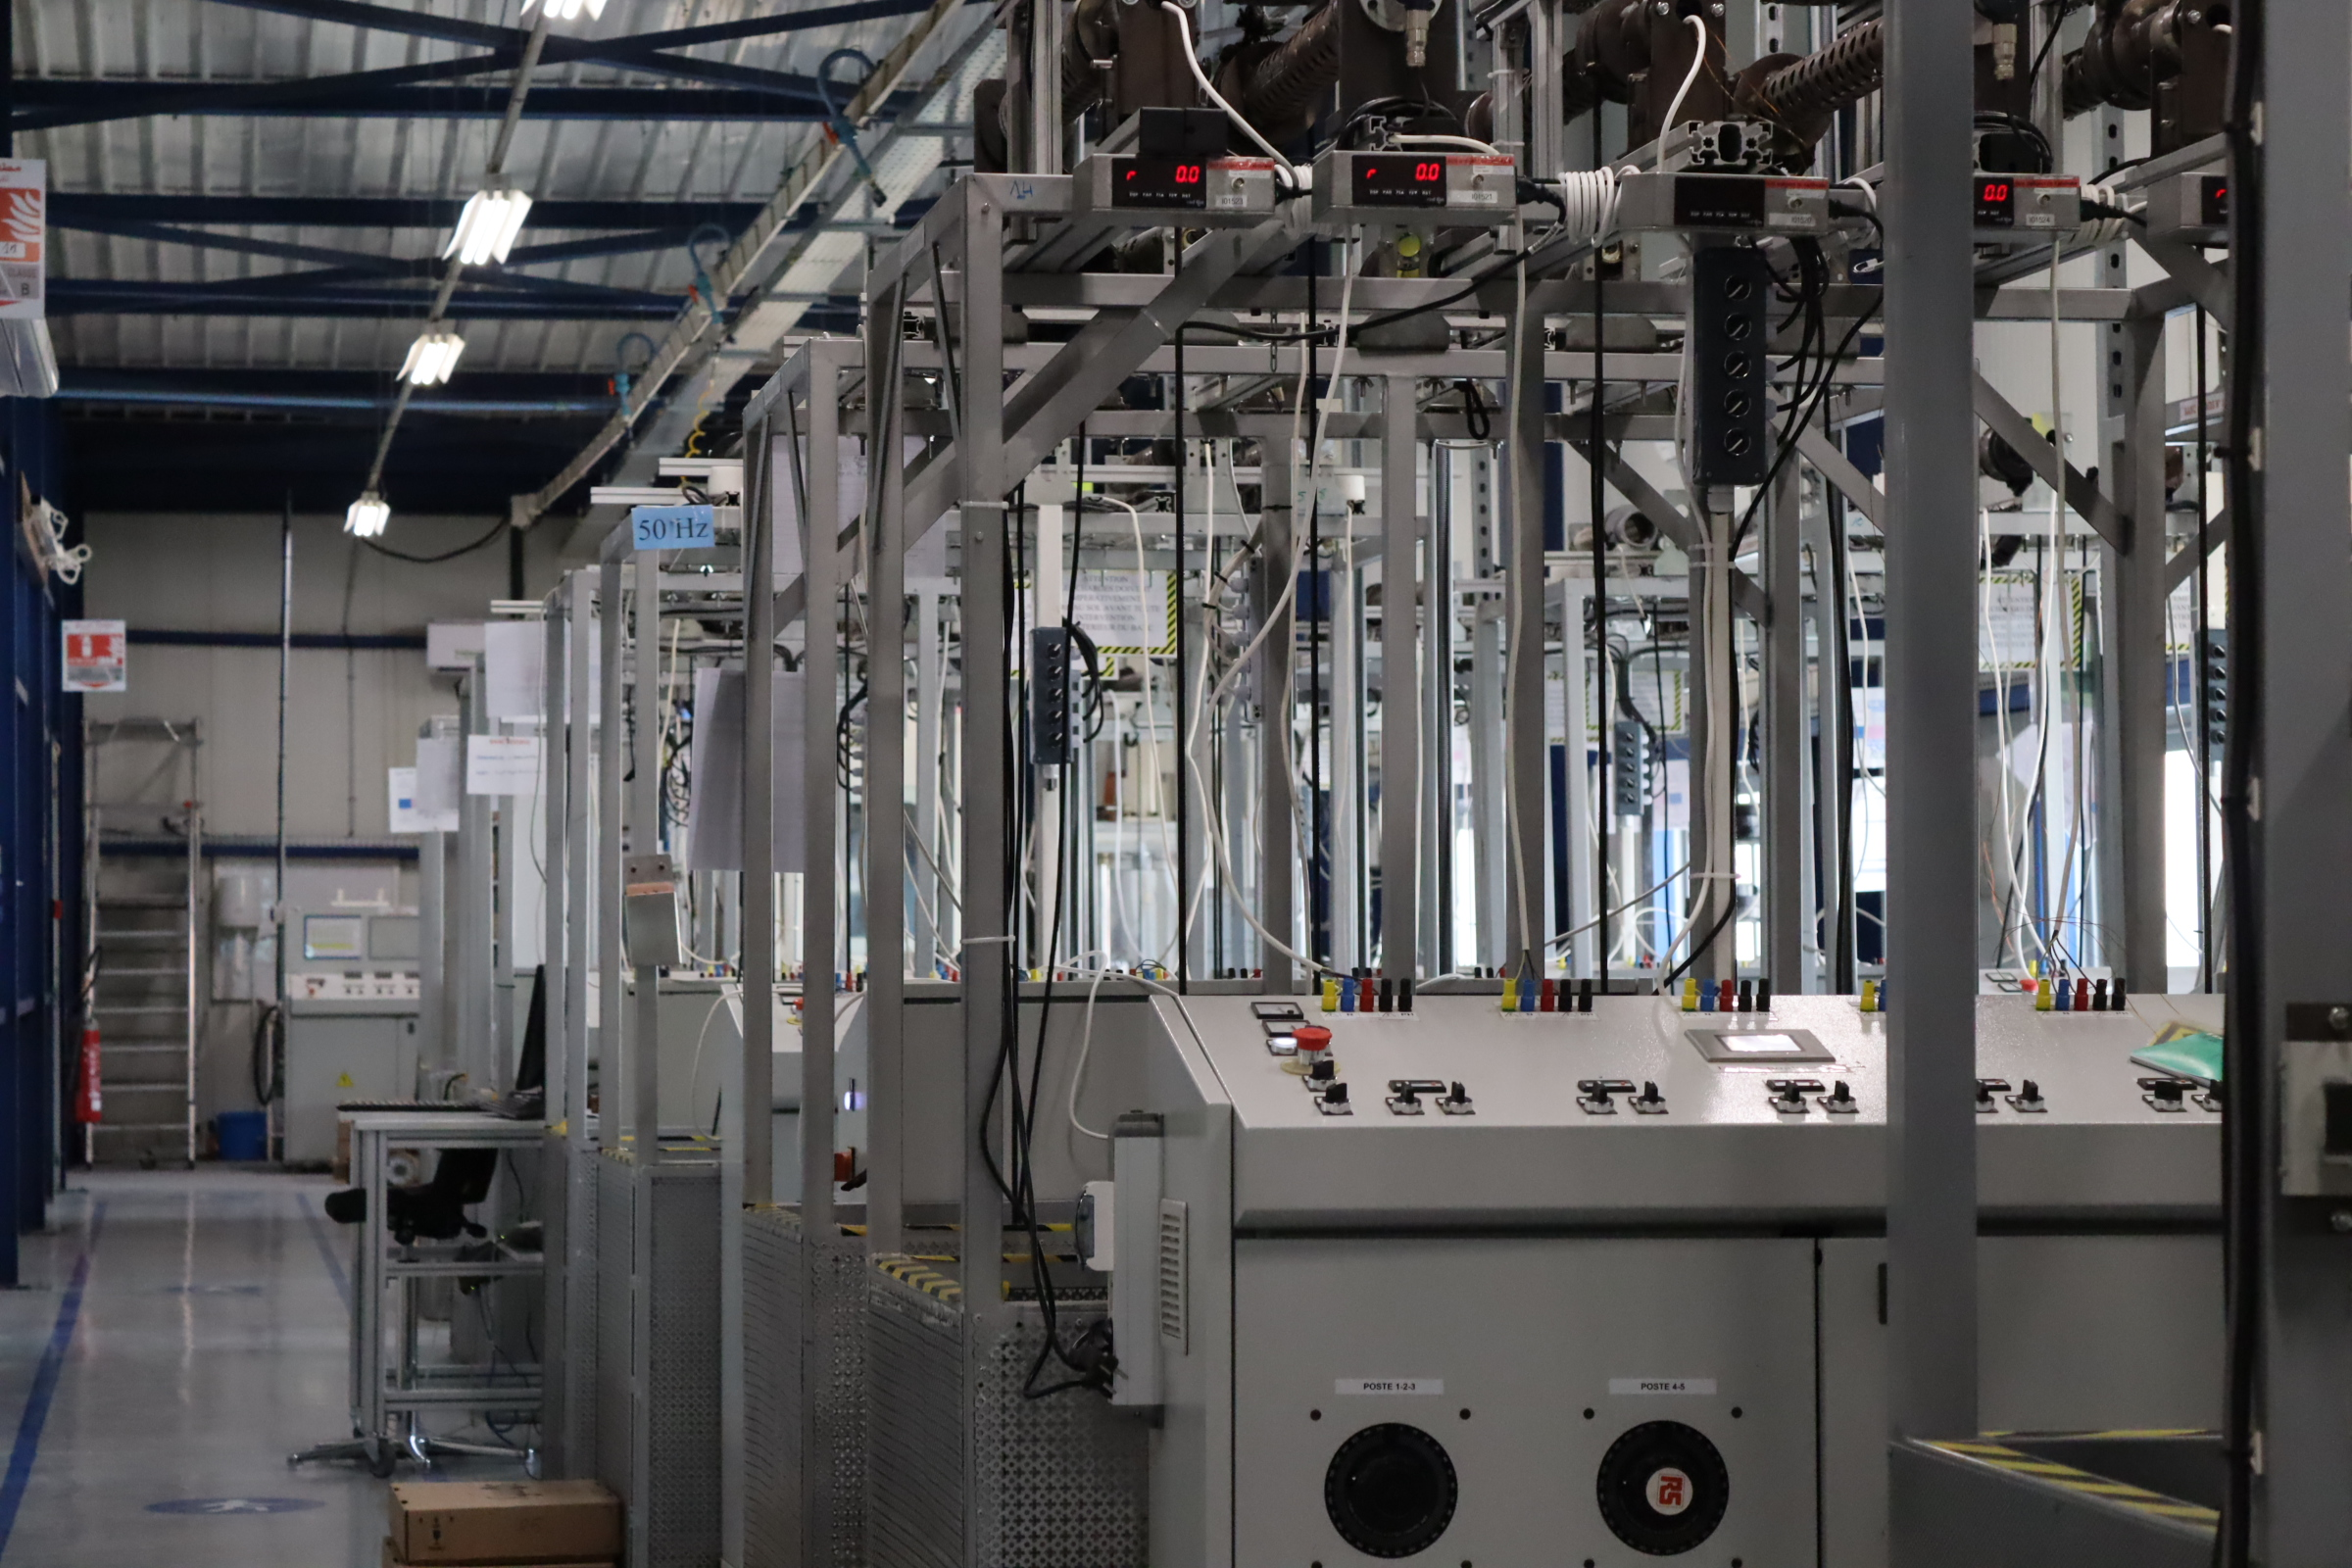
\includegraphics[width=1\textwidth]{chapters/1/img/IMG_0258.JPG}
    \caption{Somfy Zriba Lab}
    \label{fig:campus}
\end{figure}
The journey of this ambitious endeavor is detailed in this report, which highlights significant turning points, difficulties faced, and solutions put in place to change the scene of laboratory operations. 
We have created a design for the deployment of a strong and creative system that is equipped to handle the problems of the contemporary world by investigating cutting-edge technology and modifying industry best practices.
In these pages, we examine the differences and similarities between typical laboratory work and work carried out with LAB.E.S. We look at how it affects productivity, workflow, and test result quality. We will demonstrate the strategic significance of this change for laboratory operations in the future by examining the observable advantages and measurable gains.
Our dedication to quality and our common goal of innovation in laboratory management are evident in this report. It provides a useful viewpoint on both the prospects presented by the digitalization of labor and the difficulties we encounter in achieving this goal in a dynamic industrial setting.









